\documentclass[letterpaper, 10 pt, conference]{ieeeconf} 
\IEEEoverridecommandlockouts 
\overrideIEEEmargins                                      % Needed to meet printer requirements.
\usepackage{booktabs}
\usepackage{subfigure}
\usepackage{natbib}
\usepackage{graphicx}
\usepackage[ruled]{algorithm2e}
\title{\LARGE \bf
Interpreting Multimodal Referring Expressions in Real Time}
\author{Miles Eldon, David Whitney, Stefanie Tellex\\Brown University}


\usepackage{amsfonts, amssymb, amsmath}
\usepackage[usenames,dvipsnames]{color}
\newcommand{\stnote}[1]{\textcolor{Blue}{\textbf{ST: #1}}}
\newcommand{\menote}[1]{\textcolor{Red}{\textbf{ME: #1}}}

\begin{document}

\maketitle
\thispagestyle{empty}
\pagestyle{empty}

\begin{abstract}
Robots that collaborate with humans must be able to identify objects
used for shared tasks, for example tools such as a knife for
assistance at cooking, or parts such as a screw on a factory floor.
Humans communicate about objects using language and gesture, fusing
information from multiple modalities over time.  Existing work has
addressed this problem in single modalities, such as natural language
or gesture, or fused modalities in non-realtime systems, but a gap
remains in creating systems that simultaneously fuse information from
language and gesture over time.  To address this problem, we define a
multimodal Bayes' filter for interpreting referring expressions to
objects.  Our approach outputs a distribution over the referent object
at 14Hz, updating dynamically as it receives new observations of the
person's spoken words and gestures.  This real-time update enables a
robot to dynamically respond with backchannel feedback while a person
is still communicating, pointing toward a mathematical framework for
human-robot communication as a {\em joint activity}~\citep{clark96}.
Moreover, our approach takes into account rich timing information in
the language as words are spoken by processing incremental output from
the speech recognition system, traditionally ignored when processing a
command as an entire sentence.  It quickly adapts when the person
refers to a new object.  We collected a new dataset of people
referring to objects in a tabletop setting and demonstrate that our
approach is able to infer the correct object with 90\% accuracy.  Additionally, we
demonstrate that our approach enables a Baxter robot to provide
back-channel responses in real-time.
\end{abstract}

\section{INTRODUCTION}

In order for humans and robots to collaborate in complex tasks, robots
must be able to understand people's references to objects in the
external world.  For example, a robotic cooking assistant might fetch
ingredients and tools, while a robotic factory assistant could deliver
a part or a hospital robot could deliver water to a bedridden patient;
Figure~\ref{fig:example} shows a robot handing a tool to an engineer.
To refer to objects, people use a combination of language, gesture,
and body language such as eye gaze and pointing.  People provide these
signals continuously, and a person's reference can quickly change
based on new information about the domain.  Moreover, a human listener
responds to these signals as they are given using {\em backchannels},
for example nodding their head when they understand and looking
confused or interrupting to ask a question when they do not.
\citet{clark96} refers to this continuous dance as {\em joint
  activity} and compares language use to playing a duet because of its
collaborative nature, where both parties act to establish common
ground and reduce uncertainty.  Language and gesture co-occur and the
relative timing of speech and gesture is critical for accurate
understanding.  Responding quickly to a person's input makes
interaction more fluid and enables a robot to provide back-channel
feedback based on its ability to understand: when it is confident, it
can indicate that it is confident, and when it is unsure, it can
indicate that as well.  This backchannel feedback could elicit
appropriate responses from the person: they will move to the next task
when the robot understands, or provide more information to
disambiguate when the robot is confused.


Despite the importance of real-time response to multi-modal input,
existing unimodal models do not integrate information from language
and gesture~\citep{matuszek14, tellex11, kollar10} , even though
people fluidly use language and gesture together.  Approaches that
fuse information from language and gesture~\citep{matuszek14} do not
take into account that information appears to the system over a period
of time.  These approaches make it impossible for a robot to provide
back-channel feedback, because of the length of time required to
interpret the communication and because of the inability to interpret
partial utterances.

\begin{figure}
\centering
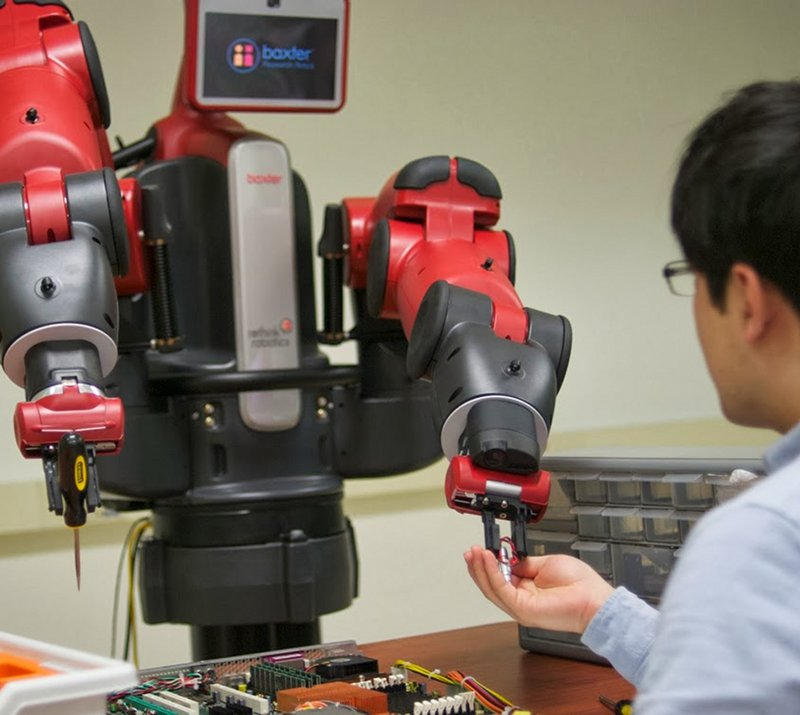
\includegraphics[width=1\linewidth]{figures/baxter_scene_cropped.jpg}
\caption{Robots that collaborate with people need to understand their
  references to objects in the environment.  For example, if a person
  asks for a tool using language and gesture, the robot needs to
  interpret the person's reference in order to pick up the correct
  tool.\label{fig:example}}
\end{figure}



To provide a foundation for these capabilities, we propose a Bayes'
filtering approach for interpreting multimodal information from
language and gesture~\citep{thrun08}.  Our framework relies on a
factored observation probability that fuses information from language,
hand gestures, and head gestures in real time to continuously estimate
the object a person is referring to in the real world.  We demonstrate
our model in simulation, as well as providing quantitative results on
a real-world RGB-D corpus of people referring to objects in the
environment.  These results demonstrate that our approach quickly and
accurately fuses multimodal information in real time to continuously
estimate the object a person is referencing.  Additionally, we
demonstrate a robot providing backchannel responses in real-time to a
person's language and gesture input.

\begin{figure*}
\centering
\subfigure[Ambiguous gesture.\label{fig:confused}]{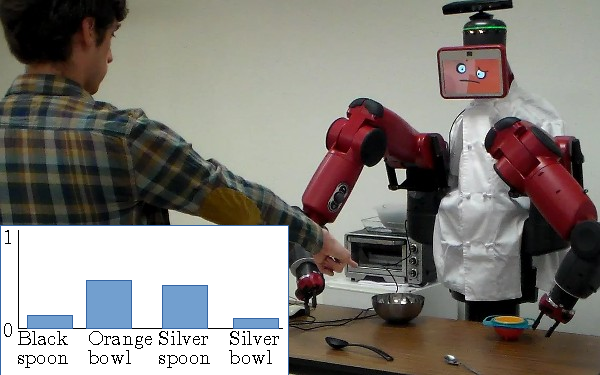
\includegraphics[width=0.49\linewidth]{figures/cartoon1.pdf}}
\subfigure[Clarification with language.\label{fig:clarified}]{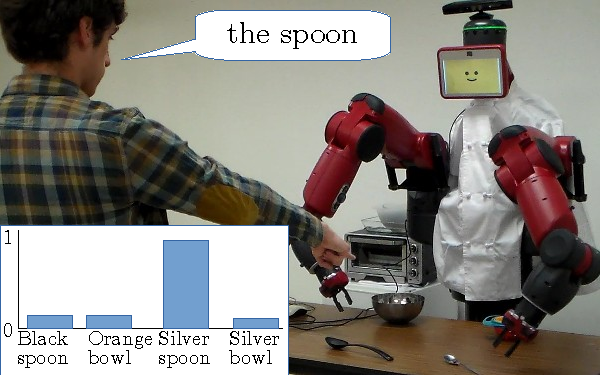
\includegraphics[width=0.49\linewidth]{figures/cartoon2.pdf}}
\caption{After an ambiguous gesture, the model has a uniform
  distribution between two objects (a).  The robot responds by
  indicating confusion.  Clarification with language causes a
  probabilistic update leaving the model highly confident it has
  inferred the correct object (b).  The robot responds by smiling and
  pointing to the correct object. \label{fig:cartoon}}
\end{figure*}

\section{RELATED WORK}

\citet{clark96} proposed that conversation is a {\em joint activity},
a coordinated, collaborative processes akin to playing a duet or
performing a waltz.  The two participants must establish {\em common
  ground}.  Common ground refers to the process of two conversational
participants establishing joint understanding about the beliefs of the
others\footnote{Note that common ground is in dialog is distinct from
  {\em symbol grounding} proposed by~\citet{harnad90}, which is the
  problem of mapping from language to aspects of the external world.}.
To establish common ground, people use {\em backchannel} feedback,
such as head nods, looks of confusion, as well as explicit request for
clarification such as asking a question.  These mechanisms enable the
participants in a conversation to engage in a feedback loop to
iteratively establish common ground as the conversation progresses.
Our approach for interpreting language and gesture in real time
provides a foundation for producing backchannel feedback with a robot,
pointing toward increased robustness as a person and robot iteratively
establish common ground and actively communicate to reduce errors.

A large body of work focuses on language understanding for
robots~\citep{macmahon06, dzifcak09, kollar10, matuszek12}.  This work
does not take into account the continuous nature of natural language
input, and requires sentences or at least chunks of words
understanding can take place.  Our approach, in contrast, incorporates
information from each word as it is processed by the speech
recognition system, integrating word information over time and fusing
it with gesture information.  \citet{guadarrama14} presents a
framework for interpreting open-domain references to objects but
focuses on interpreting language rather than language combined with
gesture.  \citet{cantrell10} presented a framework for understanding
language incrementally in real time dialog but did not use gesture and
did not use a corpus-based evaluation.  Our approach is related to
\citet{holladay14} but focuses on interpreting a person's gestures
rather than enabling a robot to generate pointing gestures.

Many existing approaches for interpreting gesture rely on fixed
vocabularies of gesture, such as ``stop'' or
``follow''~\citep{waldherr00, marge11} without a principled way for
fusing information from language and gesture.  Our work unifies
language and gesture interpretation into a single mathematical
framework, and focuses on parameterized gestures such as pointing.






\citet{matuszek14} presented a multimodal framework for interpreting
unscripted references to tabletop objects using language and gesture.
Our approach similarly focuses on tabletop objects but uses language,
gesture, and head pose, and integrates these disparate data sources
continuously over time using a Bayes' filtering framework.  This
approach enables the robot to continuously process new information and
produce an estimate that converges over time to the correct object as
new information is observed from the person.  

POMDP-approaches to dialog~\citet{young13, young10} have been extended
to incorporate gesture and noise models, and our approach is related
to these types of belief updates.  We are eager to explore enabling a
robot to adaptively respond to its estimate of which object a person
is referring to, leading to backchannels.

\citet{dragan13} created a framework enabling a robot to produce
gesture.  Similarly, \citet{tellex14} described an approach for
enabling a robot to generate language by inverting a semantics
framework.  Our long-term aim is that by combining these types of
generation approaches with real-time understanding, the robot will
produce back-channel feedback that closes the loop of dialog and
enable it to participate in dialog as a joint activity.

\section{TECHNICAL APPROACH}



Our aim is to estimate a distribution over the object that a person is
referring to given language and gesture inputs.  We frame the problem
as a Bayes' filter~\citep{thrun08}, where the hidden state,
$x \in \mathcal{X}$, is the the object in the scene that the person is
currently referencing. The robot observes the person's actions and
speech, $\mathcal{Z}$, and at each time step estimates a distribution
over the curren state, $x_t$:
\begin{align}
  p(x_t | z_0 \dots z_{0:t})
\end{align}


To estimate this distribution, we alternate performing a time update
and a measurement update.  The time update updates the belief that the
user is referring to a specific subset of objects given previous
information:
\begin{align}
p(x_t | z_{0:t-1}) = \int p(x_t|x_{t-1})\times p(x_{t-1} | z_{0:t-1}) \text{d}x_{t-1}
\end{align}

The measurement update combines the previous belief with the newest observation to update each belief state: 
\begin{align}
p(x_t |z_{0:t}) = \frac{p(z_t | x_t) \times p(x_t | z_{0:t-1})}{p(z_t | z_{0:t-1})} \\\propto p(z_t | x_t) \times p(x_t | z_{0:t-1})
\end{align}



\subsection{Prediction Model}
We assume that a person is likely to continue referring to the same
object, but at each timestep has a small probability, $c$, of
transitioning to a different object: 

\begin{align}
p(x_t | x_{t-1}) = \left\{  \begin{array}{ll}
1-c &\mbox{if } x_t = x_{t-1}\\
c &\mbox{otherwise}
\end{array}\right.
\end{align}

This assumption means that the robot's certainty slowly decays over
time, in the absence of corroborating information, converging to a
uniform distribution.  It enables our framework to integrate past
language and gesture information but also quickly adapt to new,
conflicting information because it assumes the person has changed
objects.


\subsection{Observation Model}

We assume access to an observation model of the form:
\begin{align}
p(z_t | x_t)
\end{align}

Observations consist of a tuple consisting of a person's actions,
$\langle l, r, h, s\rangle $ where:
\begin{itemize}
	\item $l$ represents the observed origin ($l_o$) and vector ($l_v$) for the left arm.
	\item $r$ represents the observed origin  ($r_o$) and vector ($r_v$)  for the right arm.
	\item $h$ represents the observed origin  ($h_o$) and vector ($h_v$)  for head.
	\item $s$ represents the observed speech from the user,
          consisting of a list of words.
	\end{itemize}

Formally, we have:
\begin{align}
p(z_t | x_t) &= p(l, r, h, s | x_t)\\
\intertext{We factor assuming that each modality is independent of the others given the state (the true object that the person is referencing):}
p(z_t | x_t) &= p(l | x_t) \times p(r | x_t) \times p(h | x_t) \times p(s | x_t)
\end{align}

\noindent The following sections describe how we model each type of
input from the person.

\noindent{\bf Gesture.}  We model pointing gestures as a vector
through three dimensional space. We calculate the angle between the
gesture vector and the vector from the gesture origin to the mean of
each cluster, and then use the PDF of a Gaussian ($\mathcal{N}$) with variance ($\sigma$) to determine the weight that should be
assigned to that object. We define a function $\mbox{A}(o, p_1, p_2)$ as the
angle between the two points, $p_1$ and $p_2$ with the given origin,
$o$.  Then 
\begin{align}
p(l | x_t) \propto \mathcal{N}(\mu_l=0, \sigma_l,A(l_o, l_v, x_t))\\
p(r | x_t) \propto \mathcal{N}(\mu_r=0, \sigma_r,A(r_o, r_v, x_t))
\end{align}

If the person's arm is more than a certain angle away from the table,
we assume they are referring to none of the objects, and perform an
update.  As a result, these gestures do not effect the robot's
estimate of the objects being referenced.

\noindent{\bf Head Pose.}
Head pose is modeled in the same manner as arm gestures.
\begin{align}
p(h | x_t) \propto \mathcal{N}(\mu_h=0, \sigma_h,A(h_o, h_v, x_t))
\end{align}


\noindent{\bf Speech.}  We model speech as a bag of words. We
take the words in a given speech input and count how many words in
this text match descriptors (denoted $x_d$) of specific objects.
\begin{align}
p(s |x_t) = \displaystyle \prod_{w \in s} p(w | x_t)
\end{align}


\subsection{Null Words and Gesture}

To account for continuous gesture and non-continuous speech input, we
have both null poses and speech.  When no words are spoken, we assume
a null word which has a uniform distribution over the objects.  This
effect means that spoken words cause a discrete bump in probability
according to the language model, which then decays over time. While
gesture remains a continuous input throughout the entire interaction,
many gestures have little or no meaning. To allow for these without
overloading the model with noise, we also calculate the angle between
each arm vector and each foot. If the angle between the arms and a
foot is smaller than the angle between the arms and any object, we
assume that the user is in a resting pose, and treat that gesture as
indicating uniform probability over all states.

\subsection{Model Parameters}
We tuned model parameters by hand.  We considered collecting and
annotating a data set to train the model parameters, but we found our
initial process to be quite accurate. We generated the language model
by hand, adding to it based on results of our pilot
studies. \stnote{We should say: ``After our initial tuning, we fixed
  model parameters, and results reported in the paper all use the same
  fixed set of parameters.''  Is that true?}  We expect that as we add
larger sets of objects, a language model trained using data from
Amazon Mechanical Turk or other corpora will be necessary to increase
robustness over a larger set of objects.  

In our experiments, we had the following parameters: the transition
probability, $c$ was 0.0005. This was determined to give an object
that has 100\% confidence an approximately 10\% drop in confidence per
second with all null observations.  Standard deviation for the
Gaussian used to model probability of gesture, $\sigma_l$,
$\sigma_r$, and $\sigma_h$ was 1.0 radians. We found that this
standard deviation allowed for accurate pointing, without skewing the
probabilities during an arm swing.  The language model consisted of
XXX\stnote{Fill in how many words. Replace ``relativly small'' with
  the exact number.} words, containing common descriptors for the
objects such as ``bowl,'' ``spoon,'' ``metal,'' ``shiny,'' etc. It
also included words that were commonly misinterpreted by the speech
recognition system, such as ``bull'' when the user was requesting a
bowl.  

%% We used unigram smootEpsilon for the language model was set to
%% 0.0001. We found that tuning this had little effect due to the size of
%% our language model. Using these descriptors and the specified epsilon,
%% we trained a unigram language model.

\begin{algorithm}
    \DontPrintSemicolon
    \KwIn{$bel(x_{t-1}), z_t$}
    \BlankLine
    \KwOut{$bel(x_t)$}
    \BlankLine
    \For{ $x_t$} {
      $\bar{bel}(x_t) = \displaystyle\prod_{x_{t-1}} p(x_t|x_{t-1})*bel(x_{t-1})$
      \BlankLine
      \textbf{if not} is\_null\_gesture(l)
      \BlankLine
      \Indp$\bar{bel}(x_t) = p(l | x_t) *  \bar{bel}(x_t)$
      \BlankLine
      \Indm\textbf{if not} is\_null\_gesture(r)
      \BlankLine
      \Indp$\bar{bel}(x_t) = p(r | x_t) *  \bar{bel}(x_t)$
      \BlankLine
      \Indm\textbf{if not} is\_null\_gesture(h)
      \BlankLine
      \Indp$\bar{bel}(x_t) = p(h | x_t) *  \bar{bel}(x_t)$
      \BlankLine
      \Indm\For{$w \in s$}{
      	$\bar{bel}(x_t) = p(w | x_t) *  \bar{bel}(x_t)$
      }
      $bel(x_t) = \bar{bel}(x_t)$

    }
    \BlankLine
\caption{Interactive Bayes Filtering Algorithm} 
\label{alg:algorithm}
\end{algorithm}

Algorithm~\ref{alg:algorithm} shows pseudocode for our approach, while
Figure~\ref{fig:cartoon} shows an example of the system's execution.
The person's gesture is ambiguous, and the system initially infers an
approximately bimodal distribution between the orange bowl and silver
spoon.  The robot indicates it has not understood by showing a
confused face.  This reaction elicits a disambiguating response from
the person, who says, ``the spoon.''  The model incorporates
information from language and infers the person is referring to the
silver spoon.  The robot indicates it has understood with a facial
expression and by pointing to the correct object.  Note that the
person's linguistic response was itself ambiguous, but provided
complementary information to the person's gesture, leading to overall
success at interpreting their intent.

Although in this example we are demonstrating the approach at two
specific timesteps, the system is updating its distribution
continuously, enabling it to fuse language and gesture as it occurs
and quickly updating in response to new input from the person, verbal
or nonverbal.  Our approach runs at 14Hz, including a 30Hz sleep
cycle, on an Asus machine with 8 2.4 GHz Intel Cores that is also
performing all perceptual and network processing. 

\section{EVALUATION}

We evaluated our model in simulation, comparing the full model to
versions without multimodal information.  Additionally we assessed its
performance on an RGB-D audio and video corpus of people referring to
objects.  Finally we created an end-to-end robotic demonstration,
demonstrated in the video attachment to our paper, and available
online\footnote{video reference}.

\subsection{Simulation Results}

We evaluated our approach in simulation by generating data from the
model and assessing its accuracy at estimating the object being
referenced.  We generated simulated pointing data for each hand, the
face, as well as spoken utterances at each timestep according to the
model parameters.  We then used these parameters to update the
system's estimate of the object being referred to.
Table~\ref{table:sim_results} shows the results.  Our accuracy metric
is the fraction of time that the robot is pointing at the correct
object.  We report performance using language alone, gesture alone,
and language combined with gesture.  These results demonstrate that
the system is successfully able to fuse multi-modal information to
achieve higher accuracy than each modality alone, but do not show
performance in the real world.  To assess robustness to signal noise,
we used two different levels of variance, demonstrating that even when
the signal is highyl noisy, our approach is able to fuse information
across modalities to improve performance.

\begin{table}
\centering
\caption{Simulation Results\label{table:sim_results}}
\begin{tabular}{lcr}
\toprule
& $\sigma^2 = 0.5$ & $\sigma^2 = 1.0$\\
Language alone &  36.5\% & 37\%\\
Head alone & 50.9\% & 35.8\%\\
Arms alone & 62.4\% & 42.1\%\\
Language and gesture &  65.7\% & 54.1\%\\
\bottomrule
\end{tabular}
\\
\stnote{Need to add results for head, arms, and language in simulation}
\end{table}

\subsection{Real-World Corpus-Based Results}

\begin{figure}
\centering
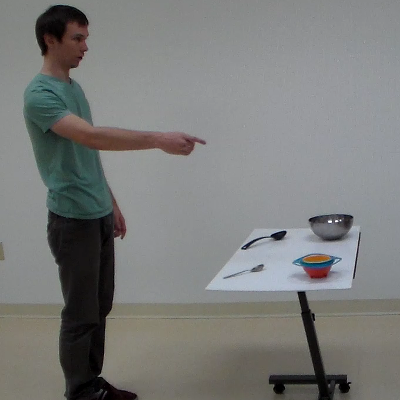
\includegraphics[width=0.5\linewidth]{figures/dataset.png}
\caption{Scene from our data collection environment.\label{fig:corpus_scene}}
\end{figure}

Our real-world experiments measured our algorithm's performance when a
person referred to an object visually and with gesture.  The subject
stood in front of a table with four objects placed approximately one
foot apart, forming four corners of a square, as shown in
Figure~\ref{fig:corpus_scene}.  We instructed subjects to ask for the
indicated object in the most natural way possible, using whatever
combination of gesture and language they felt was appropriate. We
indicted the object to refer to using a laser pointer, and we
periodically shifted to a different object on a predetermined
schedule.  They wore a microphone to pick up high-quality audio, and
we tracked their body pose using the NITE tracker~\citep{openni}.  We
used the HTML5 Speech Recognition package in conjunction with Google
Chrome to recognize speech.  This package reports incremental output
as recognition proceeds, and we perform a model update each time a new
word is perceived.  We used XX subjects, and each subject participated
in YY trials, for a total of 65 trials. \stnote{Fill in numbers.}

Results showing the percent of the time the estimated most likely
object was the true object appear in Table~\ref{table:real_results}
with 95\% confidence intervals.  During a typical trial, the model
starts out approximately uniform or unimodal on the previous object
(we did not reset the model between trials.) As the subject points and
talks, the model quickly converges to the correct object.  Our first
set of results give a sense of how quickly the model converges.

To assess overall accuracy, we report the system's accuracy at the end
of a trial in \ref{table:end_real}.  Multimodal accuracy with language
and gesture is more than 90\%, demonstrating that our approach is able
to quickly and accurately interpret unscripted language and gesture
produced by a person.  We found that our head pose estimator was quite
inaccurate, performing at worse than change unimodally.  Thus overall
results that include head pose perform worse than language and
gesture.  We believe this effect is because people's head pose quickly
changes, so the signal itself is noisy, and the OpenNI head pose
estimator is also inaccurate.

\begin{table}
\caption{Real-world Results\label{table:real_results}}
\centering
\begin{tabular}{lr}
\toprule
Random & 25\%\\
Language only &  32.4\% +/- 10\%\\
Gesture only  &  73.12\% +/- 9\%\\
Head only     &  21.67\% +/- 10\%\\
Multimodal (Language and Gesture) & {\bf 81.99\% +/- 5.5\%}\\
Multimodal (All) &  64.84\% +/- 8\%\\
\bottomrule
\end{tabular}
\end{table}
%\begin{table}
%\caption{Real-world Results\label{table:real_results}}
%\centering
%\begin{tabular}{lr}
%\toprule
%Random & 25\%\\
%Language only &  32.7\% +/- 3.5\%\\
%Gesture only  &  73.31\% +/- 4\%\\
%Head only     &  23.4\% +/- 2\%\\
%Multimodal (Language and Gesture) & {\bf 80.52\% +/- 2\%}\\
%Multimodal (All) &  64.3\% +/- 3\%\\
%\bottomrule
%\end{tabular}
%\end{table}
\begin{table}
\caption{Real-world Results (End of Interaction)\label{table:end_real}}
\centering
\begin{tabular}{lr}
\toprule
Random & 25\%\\
Language only &  46.15\%\\
Gesture only  &  80.0\%\\
Head only     & 18.46\%\\
Multimodal (Language and Gesture) & {\bf 90.77\%}\\
Multimodal (All) &  61.54\%\\
\bottomrule
\end{tabular}
\end{table}

\subsection{Robotic Demonstration}

Because our approach enables a robot to quickly monitor a person's
references to an object, the robot can respond to these estimates in
real time, producing backchannel feedback that can trigger a person to
produce disambiguating language and gesture when the person does not
understand, and move on to the next task when the robot does
understand.  We demonstrate this behavior by enabling Baxter to
demonstrate its certainty about what object is being referenced, this
eliciting more feedback from the person.  When the robot is very
unsure, it indicates its confusion by displaying a confused face,
shown in Figure~\ref{fig:confused}.  The look of confusion triggers a
disambiguating response from the person; this response causes the
model to update and the robot responds by looking confident and moving
its arm to point to the correct object.  The video shows this
behavior. \stnote{Fill in a link to the video.}

\section{CONCLUSION}

We have demonstrated a Bayes' filtering approach to interpreting a
person's multimodal language and gesture references to objects
continuously in real time.  Our approach enables a robot to understand
a person's references to objects in the real world.  This paper
represents steps toward continuous language understanding and the
vision presented by \citet{clark96} of language as joint activity.

In the future we plan to expand our language model to incorporate
models of compositional semantics and lower-level visual features so
that the robot is not limited to prespecified object models.
Additionally we aim to enable the robot to generate back-channel
feedback based on its model using a POMDP framework, ultimatly aiming
to demonstrate that by providing appropriate backchannels, the robot
elicits disambiguating responses from the person, increasing overall
speed and accuracy of the interaction.  \citet{dragan13} created a
framework for generating legible gesture, and we anticipate that
enabling a robot to respond by pointing as in \citet{holladay14} when
it is sure and reflecting its confusion when it is unsure will enable
the human-robot dyad to increase efficiency by naturally eliciting
more information when the robot is confused and indicate that the
person can move on when the robot has understood.  We also plan to
extend our approach beyond a unigram language model so that it
supports models of compositional semantics by embedding a parsing
chart into the state~\citep{jurafsky95, earley70}.  These methods will
enable the robot to understand nested referring expressions such as
``the bowl on the table'' incrementally.  Finally, we aim to extend
our approach beyond just object references; a similar modeling
approach could be used to understand references to locations in the
environment, and ultimately general command interpretation. 

\bibliographystyle{abbrvnat}
\bibliography{main}



\end{document}

